\documentclass[12pt]{report}

\usepackage[left=0.75in, right=0.75in, top=0.75in, bottom=0.75in]{geometry}
\setlength\parindent{0pt}

\usepackage{graphicx, amsmath,anonchap,tabularx,multicol}
\usepackage{wrapfig}

\usepackage{enumitem}
\setlist{noitemsep}
\setlist{nolistsep}

\newenvironment{boxe}
    {\begin{center}
    \begin{tabular}{|p{0.9\textwidth}|}
    \hline\\
    }
    { 
    \\\\\hline
    \end{tabular} 
    \end{center}
    }

\begin{document}
%%PAGE 1%%
\begin{tabular*}{\textwidth}{@{\extracolsep{\fill}}l l}
\textbf{Definite Integrals} \\
MATH 160\\
%\textbf{Due Friday, 10/22/18} & MATH 157\\
\hline\hline
\end{tabular*}\\
\begin{boxe}
For a continuous function $f(x)$ on the interval $[a,b]$ divided into $n$ sub-intervals, the width of each sub-interval is $\Delta x= \frac{b-a}{n}$.\\
Let $x_0,x_1,x_2,\dots,x_n$ be the $x$ values of the endpoints of each sub-interval.\\
\textbf{Right Riemann Sum}: $\displaystyle{\sum_{i=1}^{n}f(x_i)\Delta x}=f(x_1)\Delta x+f(x_2)\Delta x+\dots + f(x_n)\Delta x$\\
\textbf{Left Riemann Sum}: $\displaystyle{\sum_{i=0}^{n-1}f(x_i)\Delta x}=f(x_0)\Delta x+f(x_1)\Delta x+\dots + f(x_{n-1})\Delta x$

Notice that multiplying the height of the function by the width of the sub-interval is the same computation as calculating the area of a rectangle.  It is sometimes helpful to visualize definite integrals as an area between $f(x)$ and the $x$-axis.\\\\

Riemann Sum are just an approximation. A definite Integral will give us an exact value. Again suppose $f$ is continuous on the interval $a\leq x\leq b$. The \textbf{definite Integral} of $f$ from $a$ to $b$ is\\

$${\int_{a}^{b}f(x)\,dx=\lim_{n\rightarrow \infty}}\left(\sum_{i=1}^{n}f(x_i)\Delta x\right)$$\\
and equivalently we can use the left Riemann sum\\
$${\int_{a}^{b}f(x)\,dx=\lim_{n\rightarrow \infty}}\left(\sum_{i=0}^{n-1}f(x_i)\Delta x\right)$$\\
Where $f$ is called the \textit{integrand} and $a$ and $b$ are called the limits of integration
\end{boxe}

\section*{Interpreting Definite Integrals}
\begin{boxe}
1) Integrals are how we \textit{undo} derivatives: we can take quantities like velocity, rates of change, or quantities that measure ``how fast'' something changes and get quantities like displacement, or 
quantities that measure ``how much'' of something there is. Ex: The displacement of an object between $t=a$ and $t=b$ whose velocity is $v(t)$ can be computed with the definite integral $\displaystyle{\int_{a}^{b}v(t)\,dt}$\\\\
\begin{wrapfigure}{r}{0.20\textwidth}
    \centering
    \vspace*{-.9cm}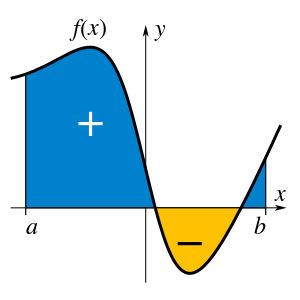
\includegraphics[width=0.16\textwidth]{300px-Integral_example.svg.png}
\end{wrapfigure}

2) Integration also measures the area between a curve and the $x$-axis. Specifically integration measures ``signed area'' or ``net area'' meaning area above the $x$-axis is positive area and area below is negative. To the right is an example of a definite integral between $a$ and $b$ and the signed area.
\end{boxe}



\end{document}
